\chapter{爆発過程の計算}
\label{chap:muller_calc}

この章では、爆発過程の計算を行った結果を書く.m\"{u}llerの論文\cite{muller}を元にPythonで数値計算のコードを書いた.ソースコードはhttps://github.com/tacohachii/supernova\_explosionにあるので参照して欲しい.

\section{データ}

weooslyの親星データ348個\cite{woosly}と,mesaで計算した親星データ107個で計算を行った.mesaのデータの分布については図\ref{fig:mesa_calc}に示す通り.wooslyの親星データの分布は図\ref{fig:woosly_data}

\begin{figure}[htbp]
  \begin{center}
    \fbox{\includegraphics[width=130mm]{./img/woosly_data.eps}}
  \end{center}
  \caption{wooslyの親星データ}
  \label{fig:woosly_data}
\end{figure}


\section{コードの質}

自作のコードの信ぴょう性を測るため,自分の計算結果とm\"{u}ller計算結果データとの比較を行った.

\begin{figure}[htbp]
  \begin{center}
    \fbox{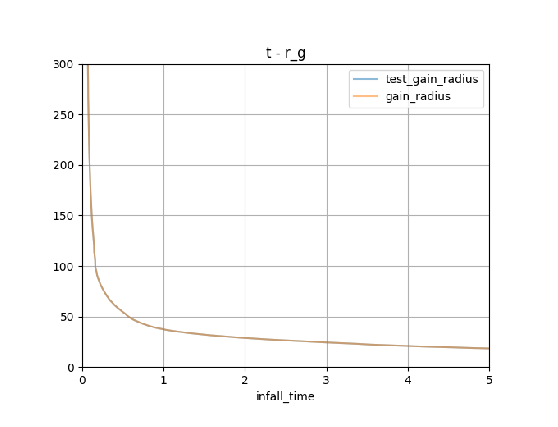
\includegraphics[width=130mm]{./img/s12M_r_g_t.eps}}
  \end{center}
  \caption{m\"{u}llerのデータとの比較($r_g$)}
  \label{fig:compare_1}
\end{figure}
\begin{figure}[htbp]
  \begin{center}
    \fbox{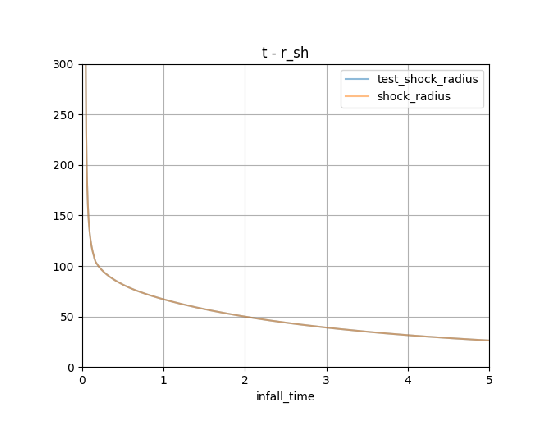
\includegraphics[width=130mm]{./img/s12M_r_sh_t.eps}}
  \end{center}
  \caption{m\"{u}llerのデータとの比較($r_{sh}$)}
  \label{fig:compare_2}
\end{figure}
\begin{figure}[htbp]
  \begin{center}
    \fbox{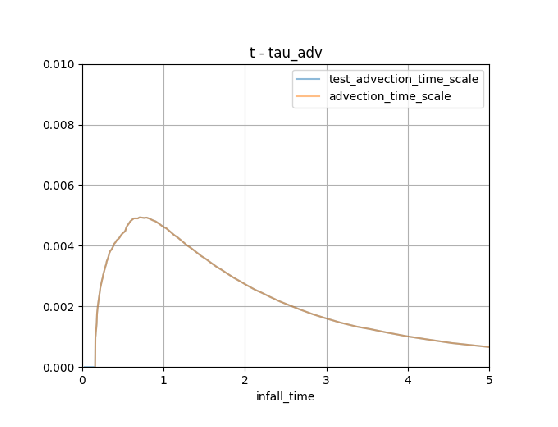
\includegraphics[width=130mm]{./img/s12M_tau_adv_t.eps}}
  \end{center}
  \caption{m\"{u}llerのデータとの比較($\tau_{adv}$)}
  \label{fig:compare_3}
\end{figure}
\begin{figure}[htbp]
  \begin{center}
    \fbox{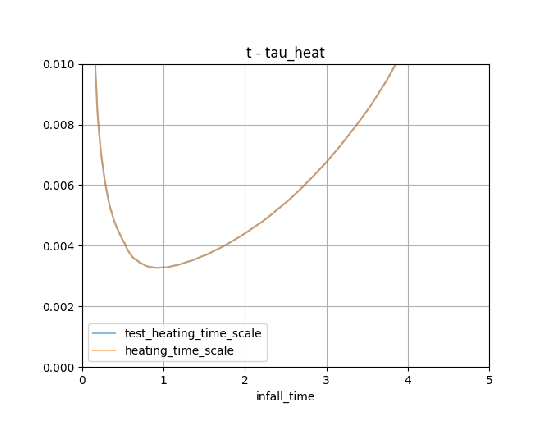
\includegraphics[width=130mm]{./img/s12M_tau_heat_t.eps}}
  \end{center}
  \caption{m\"{u}llerのデータとの比較($\tau_{heat}$)}
  \label{fig:compare_4}
\end{figure}
\begin{figure}[htbp]
  \begin{center}
    \fbox{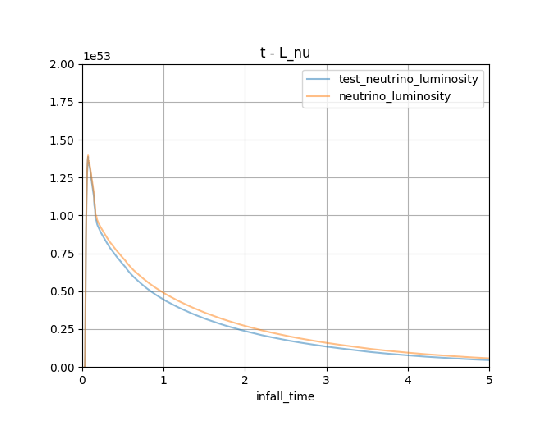
\includegraphics[width=130mm]{./img/s12M_L_nu_t.eps}}
  \end{center}
  \caption{m\"{u}llerのデータとの比較($L_{\nu}$)}
  \label{fig:compare_5}
\end{figure}
\begin{figure}[htbp]
  \begin{center}
    \fbox{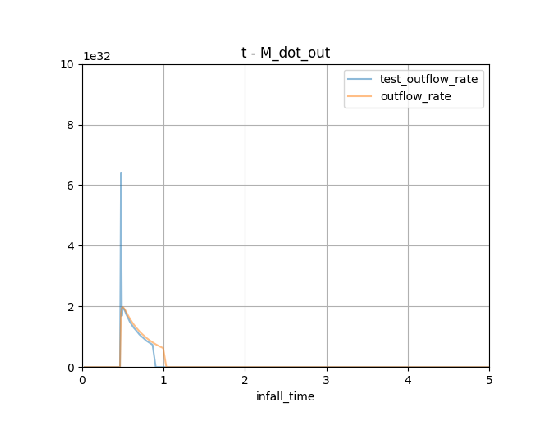
\includegraphics[width=130mm]{./img/s12M_M_dot_out_t.eps}}
  \end{center}
  \caption{m\"{u}llerのデータとの比較($\dot{M}_{out}$)}
  \label{fig:compare_6}
\end{figure}
\begin{figure}[htbp]
  \begin{center}
    \fbox{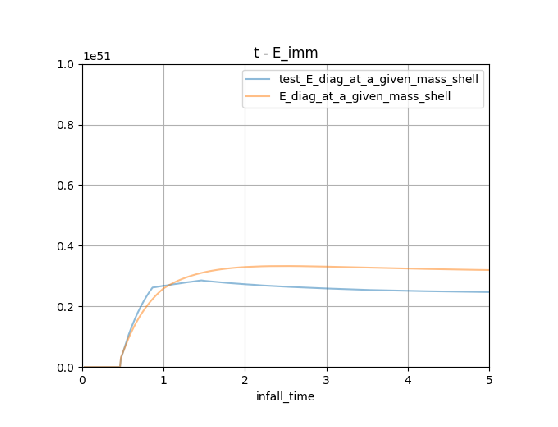
\includegraphics[width=130mm]{./img/s12M_E_imm_t.eps}}
  \end{center}
  \caption{m\"{u}llerのデータとの比較($E_{imm}$)}
  \label{fig:compare_7}
\end{figure}
\begin{figure}[htbp]
  \begin{center}
    \fbox{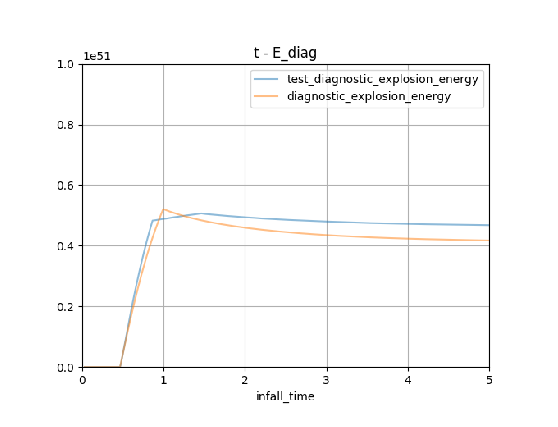
\includegraphics[width=130mm]{./img/s12M_E_diag_t.eps}}
  \end{center}
  \caption{m\"{u}llerのデータとの比較($E_{diag}$)}
  \label{fig:compare_8}
\end{figure}

\newpage

図\ref{fig:compare_1}$\sim$図\ref{fig:compare_4}までは完全に一致している.図\ref{fig:compare_5}$\sim$図\ref{fig:compare_8}では不一致の部分が目立つようになっていた.爆発段階での計算が少しずれていることが分かる.しかし,m\"{u}llerのデータの正確性が問われる状態なので大体の形が合っているということで計算の信ぴょう性は担保できたと判断した.

\section{計算例}

1つ例をあげて,$15M\sun$での計算結果の様子を紹介する.

このケースは爆発段階(Phase1)までは行くが,Phase2にはいかずにBHになる例である.

\begin{figure}[htbp]
  \begin{center}
    \fbox{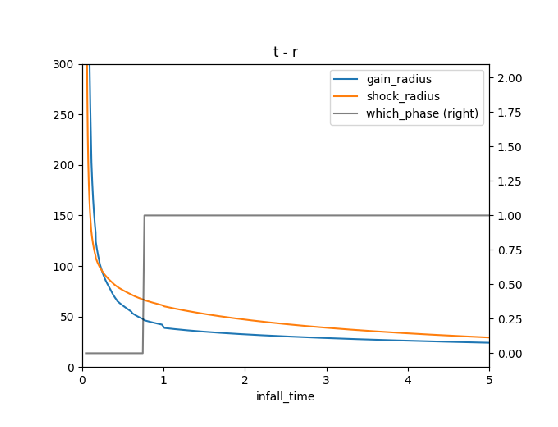
\includegraphics[width=130mm]{./img/woosley_s15.0_r_t.eps}}
  \end{center}
  \caption{ゲイン半径と衝撃波半径(woosly15.0M)}
  \label{fig:example_r_t}
\end{figure}

\begin{figure}[htbp]
  \begin{center}
    \fbox{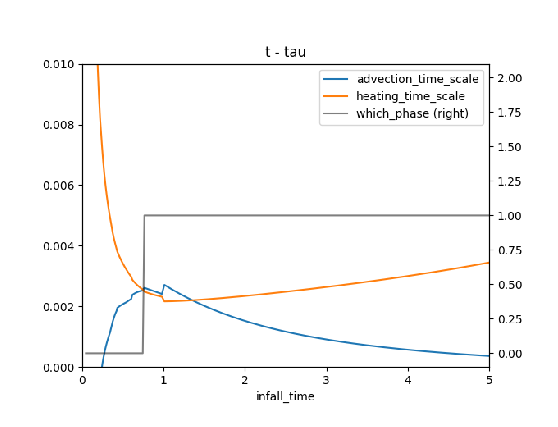
\includegraphics[width=130mm]{./img/woosley_s15.0_tau_t.eps}}
  \end{center}
  \caption{衝撃波復活の条件(woosly15.0M)}
  \label{fig:example_tau_t}
\end{figure}


\begin{figure}[htbp]
  \begin{center}
    \fbox{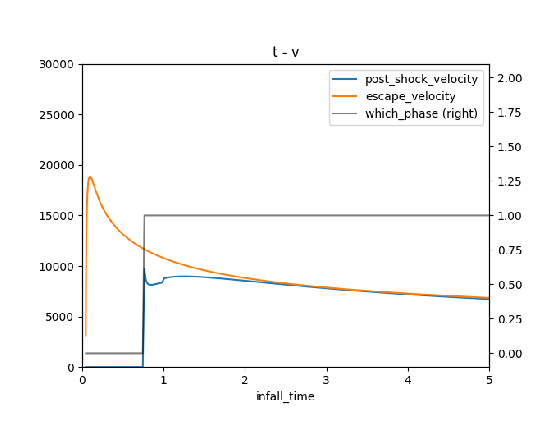
\includegraphics[width=130mm]{./img/woosley_s15.0_v_t.eps}}
  \end{center}
  \caption{Phase2へ移行できるか(woosly15.0M)}
  \label{fig:example_v_t}
\end{figure}

\begin{figure}[htbp]
  \begin{center}
    \fbox{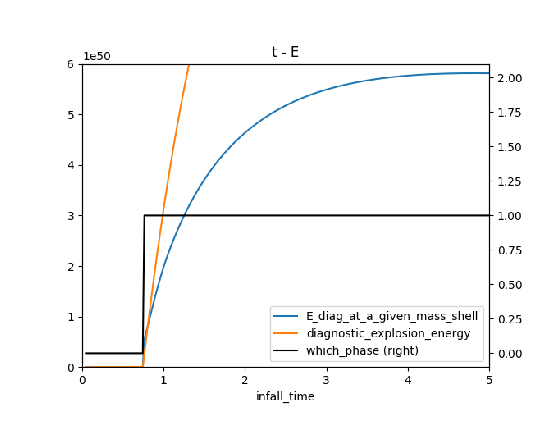
\includegraphics[width=130mm]{./img/woosley_s15.0_E_t.eps}}
  \end{center}
  \caption{爆発のエネルギー(woosly15.0M)}
  \label{fig:example_E_t}
\end{figure}

\newpage

\section{爆発結果}

全てのデータで爆発までの計算を行い.最終的な爆発のエネルギーと中性子星の質量を求めた.まずは,全体の中でどれくらいの星が爆発しているのかを見てみた.すると図\ref{fig:result_3}をみると分かるように,$25M\sun$から爆発しないという結果になった.$25M\sun$までに軸を拡大してみてみると,図\ref{fig:result_1}のようになる.右上のm\"{u}llerの論文でのグラフと比べると大きくズレがあることが分かる.


\begin{figure}[htbp]
  \begin{center}
    \fbox{\includegraphics[width=130mm]{./img/result_3.eps}}
  \end{center}
  \caption{爆発のエネルギー}
  \label{fig:result_3}
\end{figure}

\begin{figure}[htbp]
  \begin{center}
    \fbox{\includegraphics[width=130mm]{./img/result_1.eps}}
  \end{center}
  \caption{爆発のエネルギー(拡大)}
  \label{fig:result_1}
\end{figure}

\newpage
また,中性子星の質量についてもBHにならずに爆発を起こした部分なので$25M\sun$までに軸を拡大してみてみると,図\ref{fig:result_2}のようになる.これも右上のm\"{u}llerの論文上のグラフとは大きくずれていた.

\begin{figure}[htbp]
  \begin{center}
    \fbox{\includegraphics[width=130mm]{./img/result_2.eps}}
  \end{center}
  \caption{中性子星の質量(拡大)}
  \label{fig:result_2}
\end{figure}
